

\emph{Vaadin}~\cite{vaadin} es un \emph{framework} para el desarrollo de aplicaciones \emph{web} avanzadas, también conocidas como \emph{Rich-Internet Applications (RIA)}~\cite{ria}. El objetivo del paradigma \emph{RIA} es desarrollar aplicaciones \emph{web} con interfaces avanzadas que les haga asemejarse a las aplicaciones de escritorio. La principal ventaja que aporta \emph{Vaadin} es que permite escribir aplicaciones en código Java, como si fuesen de escritorio, y luego este código es transformado para que funcione en tecnologías web como HTML (\emph{HyperText Markup Language})~\cite{html}, CSS (\emph{Cascading Style Sheets})~\cite{css}, Javascript~\cite{javascript}, HTTP (\emph{Hypertext Transfer Protocol})~\cite{http} o AJAX (\emph{Asynchronous JavaScript and XML})~\cite{ajax}.

Una de las características diferenciadores de \emph{Vaadin} es que, al contrario de las librerías de JavaScript tradicionales, \emph{Vaadin} también contempla la parte del servidor, por lo se generan tanto las llamadas al servidor desde la interfaz gráfica (\emph{front-end}) como la recepción y tratamiento de esas llamadas en la parte del servidor (\emph{back-end}).

Para abstraer al usuario de elementos relacionados con HTML o Javascript, Vaadin utiliza los llamados \emph{componentes}. Un componente representa un elemento gráfico o \emph{widget}. Para el desarrollo de los componentes, Vaadin proporciona una serie de clases reutilizables que contienen los infraestructura necesaria para facilitar su traducción a código HTML y Javascript. Para crear \emph{componentes}, los desarrolladores de Vaddin deben simplemente extender estas clases.

A continuación, se explica el funcionamiento de Vaadin mediante la construcción, a modo de ejemplo, de un árbol de tareas propio de la gestión de proyectos  (Figura~\ref{fig:vaadinExampleImage}).

\begin{figure}[!tb]
	\centering
	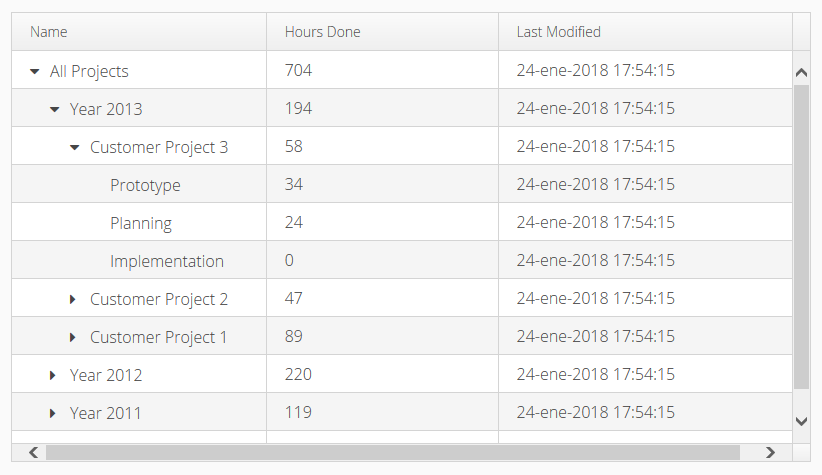
\includegraphics[width=\linewidth]{vaadinExampleImage.png}
	\caption{Árbol de Proyectos}
	\label{fig:vaadinExampleImage}
\end{figure}

\begin{figure}[!tb]
	\centering
	\begin{lstlisting}[language=Java]
	@Override
	protected void init(VaadinRequest request) {
	
	final VerticalLayout layout = new VerticalLayout();
	layout.setSpacing(true);
	layout.setMargin(true);
	
	final TreeGrid grid = new TreeGrid();
	grid.setWidth(800, Unit.PIXELS);
	grid.setHeight(450, Unit.PIXELS);
	
	JobContainer container = new JobContainer();
	grid.setContainerDataSource(container);
	
	layout.addComponent(grid);
	setContent(layout);
	}
	\end{lstlisting}
	\vspace{-15pt}
	\caption{Interfaz de Usuario Vaadin}
	\label{fig:uiVaadin}
\end{figure}

Para construir este ejemplo, en primer lugar definimos su interfaz gráfica. Para crear dicha interfaz gráfica, nos basamos en un componente gráfico, o \emph{widget}, denominado \emph{TreeGrid}  (Figura~\ref{fig:treeGrid}, Línea 8). Como puede observarse, este componente gráfico se usa directamente desde código Java, tal como se crearía una interfaz Java de escritorio, utilizando elementos propios de Java como los \emph{layouts} (Figura~\ref{fig:uiVaadin}, Líneas~4\-6) y no siendo necesario escribir nada en Javascript o HTML. Este componente mostrará los datos proporcionados por el contenedor de datos \texttt{JobContainer} (Figura~\ref{fig:uiVaadin}, Líneas~12-13).

La clase \emph{JobContainer} (Figura~\ref{fig:jobContainer}) es la que proporcionará los datos que se muestran en el \emph{grid}. Esta clase extiende de una clase de Vaadin llamada \emph{HierarchicalContainer} y se encarga de implementar toda la lógica para almacenar de forma jerárquica los nodos. Además, implementa las interfaces de Vaadin \emph{Collapsible} (Figura~\ref{fig:jobContainerCollapsible}) y \emph{Measurable} (Figura~\ref{fig:jobContainerMeasurable}), encargadas de contraer el árbol de elementos y de calcular la profundidad del elemento en la jerarquía, respectivamente.

\begin{figure}[!tb]
	\centering
	\begin{lstlisting}[language=Java]
	public class JobContainer extends HierarchicalContainer 
                               implements Collapsible, Measurable {
	
		static final String PROPERTY_NAME = "Name";
		static final String PROPERTY_HOURS = "Hours done";
		static final String PROPERTY_MODIFIED = "Last modified";
		
		public JobContainer() {
			addContainerProperty(PROPERTY_NAME, String.class, "");
			addContainerProperty(PROPERTY_HOURS, Integer.class, 0);
			addContainerProperty(PROPERTY_MODIFIED, Date.class, new Date());
			
			...	
		}
		
		private Object addItem(Object[] values) {...}
		private Object addChild(Object[] values, Object parentId) {...}
		private void setProperties(Item item, Object[] values) {...}
		private void addChildren(Object itemId) {...}
		private boolean removeChildrenRecursively(Object itemId) {...}
		
		@Override
		public boolean hasChildren(Object itemId) {...}
	}
    \end{lstlisting}
	\caption{Contenedor TreeGrid}
	\label{fig:jobContainer}
\end{figure}


\begin{figure}[!tb]
	\centering
	\begin{lstlisting}[language=Java]
	public class JobContainer
		...
		private Map<Object, Boolean> expandedNodes = new HashMap<>();
			
		@Override
		public void setCollapsed(Object itemId, boolean collapsed) {
			expandedNodes.put(itemId, !collapsed);	
			if (collapsed) {
				removeChildrenRecursively(itemId);
			} else {
				addChildren(itemId);
			}
		}
		
		@Override
		public boolean isCollapsed(Object itemId) {
			return !Boolean.TRUE.equals(expandedNodes.get(itemId));
		}
	}\end{lstlisting}
	\caption{Contenedor TreeGrid Collapsible}
	\label{fig:jobContainerCollapsible}
\end{figure}

\begin{figure}[!tb]
	\centering
	\begin{lstlisting}[language=Java]	
	public class JobContainer
	
		...
		@Override
		public int getDepth(Object itemId) {
			int depth = 0;
			while (!isRoot(itemId)) {
				depth ++;
				itemId = getParent(itemId);
			}
			return depth;
		}
	}\end{lstlisting}
	\caption{Contenedor TreeGrid Measurable}
	\label{fig:jobContainerMeasurable}
\end{figure}

Una vez creadas estas clases, utilizando \emph{Vaadin}, éstas se transforman en código \emph{HTML}, \emph{Javascript} y \emph{CSS} que pueda ser procesado en un navegador web, más una serie de llamadas \emph{AJAX} a una serie de funciones desplegadas en el servidor que se encargan de gestionar la interacción con el servidor, siguiendo la arquitectura \emph{Model-View-Presenter (MVP)}~\cite{}. La Figura~\ref{fig:vaadinMVP} muestra el funcionamiento general de este esquema.

\begin{figure}
  \centering
  \includegraphics[width=0.3\linewidth]{images/vaadin/interaction-png}
  \caption{Esquema Modelo-Vista-Presentador en Vaadin}
  \label{fig:vaadinMVP}
\end{figure}

%%==========================================================================%%
%% NOTA(Pablo): Describir lo que representa la figura que te he puesto      %%
%%              arriba                                                      %%
%%==========================================================================%%



%%==========================================================================%%
%% NOTA(Pablo): Decir esto y no decir nada es lo mismo. Te lo he encauzado  %%
%%    un poco mejor arriba.                                                 %%
%%==========================================================================%%
%% 
%% Echando un breve vistazo a la interacción cliente/servidor que facilita
%%  Vaadin, podemos explicar el código desde un punto de vista cliente y
%% servidor. El navegador, que realiza las funciones de cliente, recibe el 
%% conjunto de ficheros \emph{HTML},\emph{Javascript} y \emph{CSS} 
%% necesarios para formar la vista, este lado se encarga de cargar y 
%% visualizar dichos ficheros, así como, de recibir las acciones sobre la
%% vista para comunicarlas a la parte servidora, utilizando para ello 
%% llamadas \emph{AJAX}\cite{ajax}. Desde el punto de vista servidor,  
%% Vaadin recibe las llamadas y las trata para posteriormente recargar 
%% la vista enviando una respuesta al cliente.
%% 
%%
%% 
%% Extrapolando al ejemplo, la \emph{UI} se compilará para poder ser
%% visualizada por un navegador. El usuario al interactuar con la interfaz,
%%  enviará eventos a través del contenedor de datos, una vez finalizados 
%% los eventos, se volverá a recargar la vista para hacer visibles los
%%  cambios. De esta forma, en la parte cliente se almacenarán los ficheros 
%% \emph{HTML},\emph{Javascript} y \emph{CSS} mientras que en la parte 
%% servidora se encontrará toda la lógica.
%%
%%==========================================================================%%

Con estas indicaciones se ha creado un ejemplo sencillo de composición de elementos jerárquicos entre sí utilizando Vaadin, como podemos ver ha facilitado mucho su implementación respecto a una configuración basada en \emph{HTML} o \emph{Javascript}.

